% 2015_zhejiang_liberal_q7_fig1: oblique segment AB meeting plane alpha, P on plane
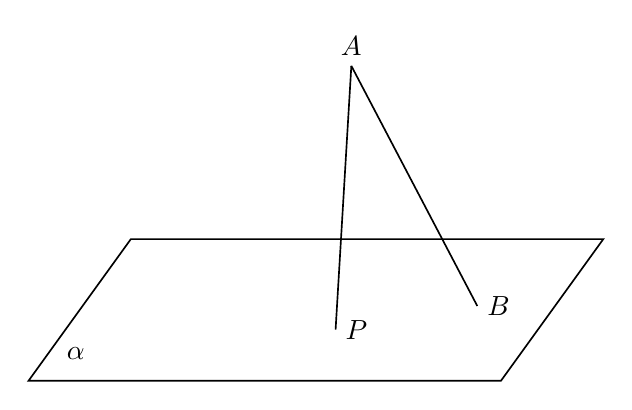
\begin{tikzpicture}[line width=0.6pt, >=stealth]
\coordinate (A) at (0.3,3.4);
% plane parallelogram
\coordinate (P1) at (-2.5,1.2);
\coordinate (P2) at (3.5,1.2);
\coordinate (P3) at (2.2,-0.6);
\coordinate (P4) at (-3.8,-0.6);
\draw (P1) -- (P2) -- (P3) -- (P4) -- cycle;
\node at (-3.2,-0.25) {$\alpha$};
\coordinate (Bp) at (1.9,0.35);
\coordinate (Pp) at (0.1,0.05);
\draw (A) -- (Bp);
\draw (A) -- (Pp);
\node[above] at (A) {$A$};
\node[right] at (Bp) {$B$};
\node[right] at (Pp) {$P$};
\end{tikzpicture}
